
This chapter presents a review in important concepts required in this development. The relationship between Flight Control Sytems (FCS) and aeroelasticity will be briefly introduced since a detailed review can be found in \citeonline{Ballesteros}. 

Next, the parameters used to evaluate actuation system performance are presented. In this section, non-linear system identification techniques such as Autoregressive with Exogenous Input (ARX) are also discussed because of their potential use in an alternative frequency response test. 

Finally, an overview on optimization problems and programming techniques is presented. For other specific details, the indicated references can be consulted.

\section{Actuator Dynamic Stiffness}

In an aircraft, the capability to turn, roll and climb ($N$, $L$ and $M$ in Figure \ref{fig:2_1_AirplaneAxis}) is provided by the Primary Flight Control System (PFCS). This system is responsible of acquiring movement commands from the pilots and executing them in a predictable and smooth fashion. Currently, most PFCS architectures rely on fly-by-wire technology to deliver the expected performance.

\begin{figure}[H]
	\centering
	\centerline{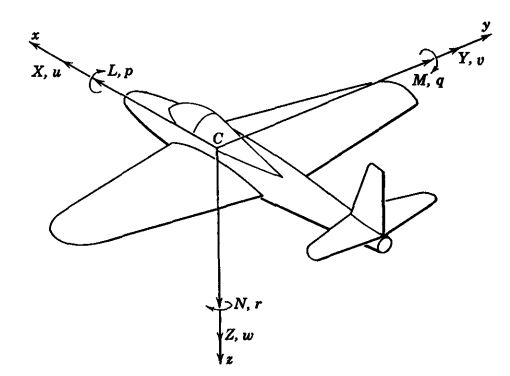
\includegraphics[width=0.7\textwidth]{Figuras/2.TheoryBackground/2-1-AirplaneAxis.jpg}}
	\caption{Notation for Aircraft Body Axes. Source: \citeonline{Etkin}}
	\label{fig:2_1_AirplaneAxis}
\end{figure}

In fly-by-wire architectures, an electronic computer receives electrical signals from sensors measuring the pilots inputs over cockpit controls. After processing this data, the computer electrically sends a position command to each primary surface actuator which is responsible to move the piston and maintain the commanded position. Usually, this task is performed by EHSAs which receive an electric position command signal and uses hydraulic power to convert the surface position command and achieve the commanded piston position.

Aircraft control surfaces are subject to aeroelastic phenomena, such as flutter, as well as other structure parts. Wright and Cooper \citeyear{Wright} define flutter as:

\begin{center}
	\textit{``(...) an unstable self-excited vibration in which the structure extracts energy from the air stream and often results in catastrophic structural failure. Classical binary flutter occurs when the aerodynamic forces associated with motion in two modes of vibration cause the modes to couple in an unfavourable manner.''}
\end{center}  

Flutter	is avoided by designing structures and other parts with appropriate stiffness at critical frequencies i.e. a surface vibration movement induced by the air stream will be small enough to avoid coupling with other vibration modes. 

The overall stiffness of a flight control surface for flutter suppression is broken down in budgets for each part of the assembly. Figure \ref{fig:2_1_DynStiff} shows an example of this distribution.

\begin{figure}[H]
	\centering
	\centerline{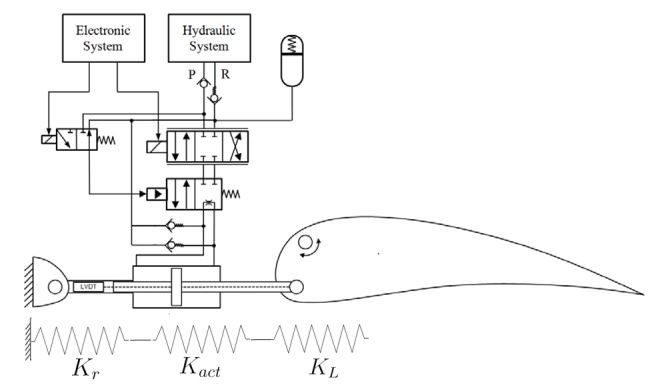
\includegraphics[width=0.7\textwidth]{Figuras/2.TheoryBackground/2-FlutterDynamicStiff.jpg}}
	\caption{Surface stiffness components. Adapted from \citeonline{Constantino}}
	\label{fig:2_1_DynStiff}
\end{figure}

The flight control surface equivalent linear dynamic stiffness ($K_{lin}$) is defined as:

\begin{equation}
\frac{1}{K_{lin}} = \frac{1}{K_r} + \frac{1}{K_L} + \frac{1}{K_{act}}
\label{eq:klin}
\end{equation}

Where $K_r$ and $K_L$ refer to structural stiffness components and $K_{act}$ is the actuator contribution to the surface dynamic stiffness.

Since flight control actuators contribute to control surface stiffness, one of the EHSA design requirements
is its dynamic stiffness.

The subject of this work is the maximization of actuator dynamic stiffness using optimization algorithms to ascertain control loop gains while maintaining compliance with time and frequency domain performance requirements. 

%\subsection{Dynamic Stiffness}

\section{Control Systems Performance}

In Flight Control Systems design, actuator control performance specifications contain time and frequency domain parameters. This section will define the parameters used in this work to assess the feasibility of each design.

\subsection{System Step Input Response}

In general, time domain performance of a system is defined based on its step response as shown in Figure \ref{fig:2_2_1_StepInputParameters} \cite{Dorf}.

\begin{figure}[H]
	\centering
	\centerline{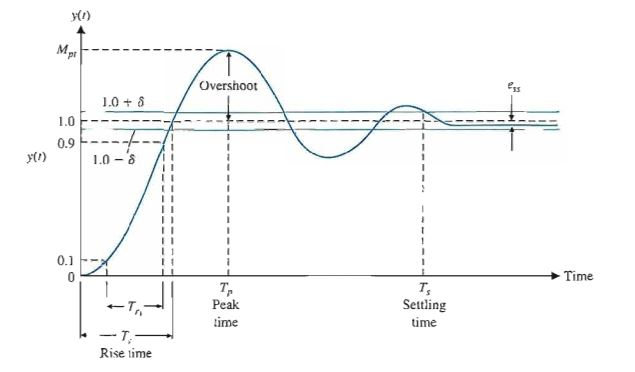
\includegraphics[width=0.9\textwidth]{Figuras/2.TheoryBackground/2-2-1-StepResponseParameters.jpg}}
	\caption{Step response of a control system. Source: Dorf and Bishop (\citeyear{Dorf})}
	\label{fig:2_2_1_StepInputParameters}
\end{figure}

The quickness of the response is measured by the rise time ($T_r$) and the peak time ($T_p$). For over damped systems the rise time is the difference between the instant where the response reaches 90\% of its final value and the instant when it reaches 10\%. The peak time is the instant when the response reaches its maximum value but this measure is not defined for over damped systems. For under damped systems the peak time is well defined and the rise time is usually taken between 0\% and 100\% of the reference input value.

The closeness of the response to the step command is determined by the overshoot, settling time and steady state error.

The response overshoot is the percentage of the final value that exceeds it in the first peak of an under damped system response. Formally, it is given by Equation \ref{eq:2_2_OvershootEquation}:

\begin{equation}
\label{eq:2_2_OvershootEquation}
O = \frac{M_p - y_s}{y_s} \times 100\%
\end{equation}

Where $M_p$ is the maximum value of the system step response and $y_s$ is the final value of the response. 

The settling time ($T_s$) is defined as the time when model response reaches and remains within a certain percentage of its steady-state value. This parameter indicates the actual time it takes the system to reach the commanded position.

The steady state error determines the response closeness to the commanded value and it is given by Equation \ref{eq:2_2_1_SteadyStateEquation}:

\begin{equation}
\label{eq:2_2_1_SteadyStateEquation}
e_{ss} = \frac{y_s - r}{r} \times 100\%
\end{equation}

Where $y_s$ is the final value of the response and $r$ is the commanded value.

%Another parameter used specially in control surface actuator systems is the actuation average rate. As defined by \citeonline{Ballesteros}, it is the surface angular travel divided by the travel time between 15\% and 85\% of the steady state value ($y_s$).

\subsection{System Frequency Response}

Figure \ref{fig:2_2_2_SystemBlockDiagram} shows a general one degree-of-freedom feedback control system.

\begin{figure}[H]
	\centering
	\centerline{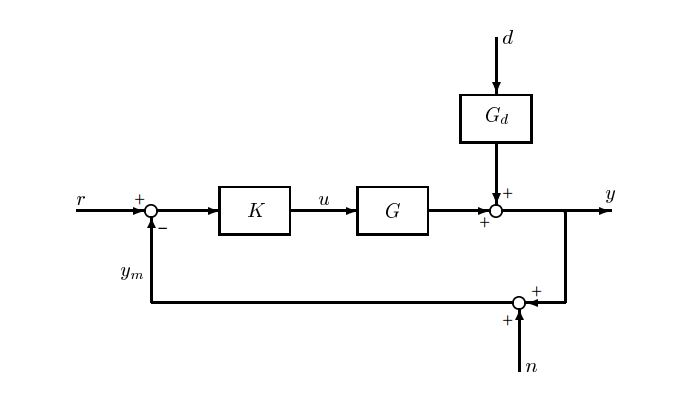
\includegraphics[width=0.9\textwidth]{Figuras/2.TheoryBackground/2-2-2-SystemBlockDiagram.jpg}}
	\caption{Block diagram of a one degree-of-freedom feedback control system. Source: Skogestad and Postlethwaite (\citeyear{Skogestad})}
	\label{fig:2_2_2_SystemBlockDiagram}
\end{figure}

Skogestad and Postlethwaite (\citeyear{Skogestad}) deduce for this general system the following relationship between reference, disturbance and noise inputs and the system output in Equation \ref{eq:2_2_2_SystemOutput}.

\begin{equation}
\label{eq:2_2_2_SystemOutput}
y = (I + GK)^{-1}GKr + (I + GK)^{-1}G_{d}d + (I+GK)^{-1}GKn
\end{equation}

Where:

\begin{description}
	\item \hspace{20pt}$r$: reference input signals;
	\item \hspace{20pt}$u$: control signals;
	\item \hspace{20pt}$d$: disturbance input signals;
	\item \hspace{20pt}$y$: system output signals;
	\item \hspace{20pt}$n$: noise input in measured signals;
	\item \hspace{20pt}$ym$: system feedback signals;
	\item \hspace{20pt}$K$: controller transfer function;
	\item \hspace{20pt}$G$: plant transfer function;
	\item \hspace{20pt}$G_d$: disturbance plant transfer function;
\end{description}

Additionally, it is defined the following terminology for transfer functions that are useful for frequency domain analysis, shown in Equations \ref{eq:2_2_2_LoopTF}, \ref{eq:2_2_2_SensitivityTF} and \ref{eq:2_2_2_CompSensitivityTF}.

\begin{equation}
\label{eq:2_2_2_LoopTF}
L = GK
\end{equation}
\begin{equation}
\label{eq:2_2_2_SensitivityTF}
S = (I + GK)^{-1} = (I + L)^{-1}
\end{equation}
\begin{equation}
\label{eq:2_2_2_CompSensitivityTF}
T = (I + GK)^{-1}GK = (I + L)^{-1}L
\end{equation}

Where:

\begin{description}
	\item \hspace{20pt}$L$: open-loop function;
	\item \hspace{20pt}$S$: sensitivity function;
	\item \hspace{20pt}$T$: complementary sensitivity function;
\end{description}

The frequency response of $L$, $S$ and $T$ may be used to establish a relationship between open-loop frequency response and system performance parameters such as gain and phase margins.

Gain margin, usually given in Decibels (dB), is the factor by which the loop gain $|L(jw)|$ may be increased before the closed-loop system becomes unstable \cite{Skogestad}. It is defined by Equation \ref{eq:2_2_2_GainMargin}.

\begin{equation}
\label{eq:2_2_2_GainMargin}
GM = 20log\left(\frac{1}{|L(j\omega_{180})|}\right)
\end{equation}

Where the phase crossover frequency $w_{180}$ is the frequency whose the phase of $|L(jw)|$ is 180 degrees.

The gain margin is important because of the real system parameters uncertainty that may cause a difference between real and modeled transfer function gains. If this difference is higher than the gain margin the system will be unstable.

Phase margin, usually given in Degrees ($°$), is the phase delay at the gain crossover frequency $w_{0dB}$ that can be introduced in the feedback loop before the closed-loop system becomes unstable. It is defined by Equation \ref{eq:2_2_2_PhaseMargin} \cite{Skogestad}.

\begin{equation}
\label{eq:2_2_2_PhaseMargin}
PM = \angle L(j\omega_{0dB}) + 180°
\end{equation}

It is also important to understand and define proper phase margin requirements to avoid unexpected instability due to system parameters uncertainty.

Sometimes is not possible to obtain these margins via Equations \ref{eq:2_2_2_GainMargin} and \ref{eq:2_2_2_PhaseMargin}, for instance, when $L(j\omega)$ is unknown. An alternative method is to use a computer model to perform simulations and obtain the system response for a sine wave input at each frequency of interest.

Considering the block diagram of Figure \ref{fig:2_2_2_SystemBlockDiagram} as this computer model, the input would be $r$ and the output of transfer function $L(j\omega)$ would be $y_m$.

In this case, the magnitude and phase delay at each frequency can be obtained by processing the input and output of these simulations. Signals $r$ and $y_m$ Fourier Transform ($R$ and $Y_m$) provide their spectrum, where the component at the frequency of interest $\omega_i$ can be obtained. 

In this case, magnitude and phase of the frequency response are given by Equations \ref{eq:2_2_2_FRMag} and \ref{eq:2_2_2_FRPhase}.

\begin{equation}
\label{eq:2_2_2_FRMag}
|L(j\omega_i)| = \frac{|Y_m(j\omega_i)|}{|R(j\omega_i)|}
\end{equation}
\begin{equation}
\label{eq:2_2_2_FRPhase}
\angle L(j\omega_i) = \angle Y_m(j\omega_i) - \angle R(j\omega_i)
\end{equation}

After obtaining magnitude and phase of $L(j\omega)$ for an adequate set of frequencies, the gain and phase margins of the control system can be obtained with Equations \ref{eq:2_2_2_GainMargin} and \ref{eq:2_2_2_PhaseMargin}.

Another alternative method to obtain gain and phase margins of a control system is to use Equations 
\ref{eq:2_2_2_MaxTSko}, \ref{eq:2_2_2_GainMarginSko} and \ref{eq:2_2_2_PhaseMarginSko} \cite{Skogestad}. This alternative will provide a minimum value for these margins. 

If the complementary sensitivity function $T$ is unknown, its frequency response can also be obtained through simulations as mentioned above using $r$ as the input and $y$ as the output.

\begin{equation}
\label{eq:2_2_2_MaxTSko}
M_T = \max_{\omega} |T(j\omega)|
\end{equation}
\begin{equation}
\label{eq:2_2_2_GainMarginSko}
GM \geq 1 + \frac{1}{M_T}
\end{equation}
\begin{equation}
\label{eq:2_2_2_PhaseMarginSko}
PM \geq 2 \arcsin \left(\frac{1}{2M_T}\right)
\end{equation}

Other useful parameters to assess frequency domain performance are the bandwidth, droop and magnitude peak. These are all obtained from the complementary sensitivity function as detailed below.

The bandwidth provides the frequency range in which control is effective. \citeonline{Dorf} defines that, in systems where the low-frequency magnitude is 0 dB, the bandwidth ($\omega_{BT}$) is the frequency in which the closed-loop magnitude response is -3 dB as per Equation \ref{eq:2_2_2_Bandwidth}. A visual representation of the bandwidth is shown in Figure \ref{fig:2_2_2_Bandwidth}.

\begin{equation}
\label{eq:2_2_2_Bandwidth}
|T(j\omega_{BT})|=-3 dB
\end{equation}

\begin{figure}[H]
	\centering
	\centerline{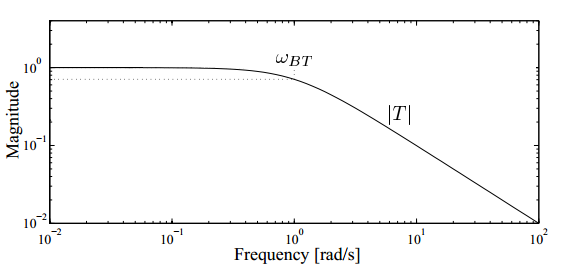
\includegraphics[width=0.7\textwidth]{Figuras/2.TheoryBackground/bandwidth.png}}
	\caption{Example of magnitude response of $T(j\omega)$. Adapted from Skogestad and Postlethwaite (\citeyear{Skogestad})}
	\label{fig:2_2_2_Bandwidth}
\end{figure}

The magnitude peak is defined by equation \ref{eq:2_2_2_MaxTSko} and can be seen in Figure \ref{fig:2_2_2_DroopPeak} which also shows the droop. The droop is the minimum value of magnitude of the frequency response between the zero and the peak frequency. Droop requirements are often defined to avoid a reduction of the bandwidth.

\begin{figure}[H]
	\centering
	\centerline{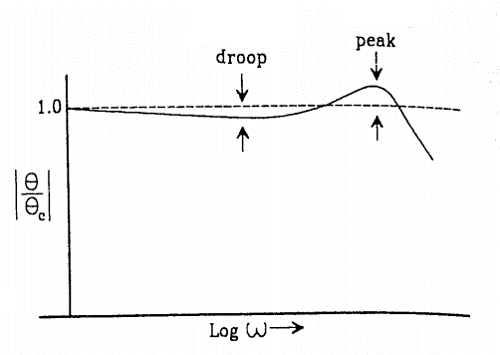
\includegraphics[width=0.6\textwidth]{Figuras/2.TheoryBackground/drooppeak.png}}
	\caption{Closed-loop frequency response droop and magnitude peak. Adapted from Stevens and Lewis (\citeyear{Lewis})}
	\label{fig:2_2_2_DroopPeak}
\end{figure}

\subsubsection{Nonlinear ARX Models}

Another method for obtaining the frequency response is through the identification of the system model. System Identification is a discipline dedicated to build mathematical models of dynamic systems based on observed data from these systems \cite{Ljung}. Many applications of this discipline focus on finding a model that describes well a system of interest so this model can be easily simulated to support the controller design process.

However, there are different uses for these techniques such as finding the frequency response of a system. Computational models can be very complex and time consuming to simulate, what burdens their use as a design tool. An option to overcome this challenge is to find a mathematical model that describes well the complex computational model and is easier to manipulate.

A mathematical model that can describe nonlinear systems is the ARX. These model consists in a set of regressors and a nonlinearity estimator, as shown in Figure \ref{fig:2_4_ARXModel}. 

\begin{figure}[H]
	\centering
	\centerline{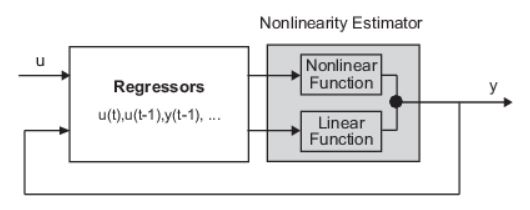
\includegraphics[width=0.6\textwidth]{Figuras/2.TheoryBackground/2-4-ARXModel.jpg}}
	\caption{ARX Model Structure. Source: \citeonline{IdtToolbox}}
	\label{fig:2_4_ARXModel}
\end{figure}

The nonlinearity estimator contains linear and nonlinear functions that act on the model regressors to give the model output \cite{IdtToolbox}. Equation \ref{eq:2_4_ARXMathModel} shows the mathematical structure of an ARX model for a single-input single-output (SISO) system.

\begin{equation}
\label{eq:2_4_ARXMathModel}
y(t) = \textbf{F}(y(t-1),y(t-2),...,y(t-n_o),u(t),u(t-1),...,u(t-(n_i-1)))
\end{equation}

Where:

\begin{description}
	\item \hspace{20pt}$y(t)$: model output at instant $t$;
	\item \hspace{20pt}$\textbf{F}$: nonlinearity estimator function whose inputs are model regressors;
	\item \hspace{20pt}$n_o$: regressor order that specifies the number of regressors from the output to predict the output;
	\item \hspace{20pt}$n_i$: regressor order that specifies the number of regressors from the input to predict the output.
\end{description}

The regressor stage introduces delays in the inputs and outputs of the model and creates an array of inputs used by the non linear estimator to generate a model output. \textbf{F} is a nonlinear function that is defined by the type of non linear estimator, such as \textit{wavelet network}, \textit{sigmoid network} and \textit{bynary tree}.

The \textit{wavelet network} estimator has a mathematical structure in which the wavelet function is applied to each regressor and is the default estimator for nonlinear ARX model identification in MATLAB. 

Estimator \textit{sigmoid network} structure is similar to the \textit{wavelet network} but the sigmoid function is applied to each regressor. Finally, \textit{tree partition} is an estimator that uses a binary tree structure to partition the regressor space and apply a linear function to each partition.

\subsubsection{Total Harmonic Distortion}

The Total Harmonic Distortion (THD) is used to quantify the level of harmonics in a waveform. In this work, it has been used to quantify how much non-linear the actuator response is in comparison to its linear component. In others words, the THD quantifies the non-linearity of the response.

The THD is defined by Equation \ref{eq:2_2_2_2_THD} \cite{Doron}.

\begin{equation}
\label{eq:2_2_2_2_THD}
THD = \dfrac{\sqrt{V_2^2+...+V_n^2}}{\sqrt{V_1^2+V_2^2+...+V_n^2}}\times 100\%
\end{equation}

Where $V_n$ is the root mean square value of the $n^{th}$ harmonic and $n=1$ is the fundamental frequency. The THD measures the ratio between the power of the harmonics and the total power of the waveform in percentage. Hence, if the THD is low, the harmonics introduced by the system do not have a major influence in the response whereas high values of THD indicate that the system output is highly distorted.

\subsection{Actuation System Frequency Domain Requirements}

Even though gain and phase margin are important parameters in control systems design, sometimes the requirements of a surface actuation system are written in terms of its closed loop frequency response. 

The need to characterize the local closed control loop of each surface actuator is due to the aircraft-level control laws that consider them as plants to be controlled. For instance, \citeonline{MIL9490} provides guidance for the definition of aircraft-level control loop gain and phase margins requirements. These requirements are broken down as frequency response budgets for each component of the aircraft control loop such as the flight control computer, digital data bus delays, actuation control loop and sensors dynamics.

Hence, during early development stages, aircraft manufacturer and supplier work together to agree a set of closed-loop performance requirements for the actuation systems so that each party can carry-on separately with design activities.

In the perspective of the aircraft manufacturer, regarding frequency domain performance, it is important to know how much delay and gain can be introduced in the aircraft-level control loop so its controllers, filters and other logics have defined restrictions. 

Additionally, the verification of gain and phase margins of the local actuation system in the real product is not practical from a development strategy standpoint. The verification of these requirements require a more complex software/firmware and even so there is a risk of the actuator reaching the mechanical stop and consuming fatigue life which is not long for primary actuators, also, it is difficult to guarantee repeatability of this test.

Therefore, it is common in the industry to specify closed-loop frequency response requirements of surface actuation systems. There are many parameters to use in these specifications such as bandwidth, magnitude peak and droop. Despite this, the frequency performance parameters selected for this work were the same used by \citeonline{Ballesteros} in order to allow a fair result comparison, they are the maximum gain at the phase crossover frequency (Closed-Loop Gain Allowance - CLGA) and the maximum phase delay at the gain crossover frequency (Closed-Loop Phase Allowance - CLPA).

For the system in Figure \ref{fig:2_2_2_SystemBlockDiagram}, CLGA and CLPA can be obtained with Equations \ref{eq:2_2_3_CLGainMargin} and \ref{eq:2_2_3_CLPhaseMargin}.

\begin{equation}
\label{eq:2_2_3_CLGainMargin}
CLGA = 20log\left(\frac{1}{|T(j\omega_{180})|}\right)
\end{equation}
\begin{equation}
\label{eq:2_2_3_CLPhaseMargin}
CLPA = \angle T(j\omega_{0dB}) + 180°
\end{equation}

Where:

\begin{description}
	\item \hspace{20pt}$T$: complementary sensitivity function;
	\item \hspace{20pt}$\omega_{180}$: phase crossover frequency;
	\item \hspace{20pt}$\omega_{0dB}$: gain crossover frequency;
\end{description}

Using the CLGA as a requirement prevents the occurrence of high gains in high frequencies and as a result large bandwidths are avoided. This is desired since large bandwidths are related to a high noise sensitivity. Additionally, the CLPA is useful for guaranteeing a maximum phase delay at the gain crossover frequency which leads to an overall reduced phase delay.

Even though these are useful metrics, it is suggested for future works to use closed-loop frequency response parameters such as bandwidth, peak magnitude and droop, which are aligned with common industry and academia practice.

\section{Optimization Problems} \label{2-3-OptimizationProblems}
%*See section 5.2 of Optimization Ref*

In general, single objective optimization problems are formulated as follows (\citeauthor{Messac}, \citeyear{Messac}; \citeauthor{Rao}, \citeyear{Rao}; \citeauthor{Fletcher}, \citeyear{Fletcher}).

\begin{equation}
\label{eq:2_2_OptimizationFormulation}
\underset{x}{\text{minimize}} f(x)
\end{equation}

Such that:

\begin{equation}
\label{eq:2_2_IneqConstOptimizationFormulation}
g(x) \leq 0
\end{equation}
\begin{equation}
\label{eq:2_2_EqConstOptimizationFormulation}
h(x) = 0
\end{equation}
\begin{equation}
\label{eq:2_2_BoundsOptimizationFormulation}
x_l \leq x \leq x_u
\end{equation}

Where:

\begin{description}
	\item \hspace{20pt}$x$: array of design variables;
	\item \hspace{20pt}$f(x)$: objective function to be minimized over the $x$ array;
	\item \hspace{20pt}$g(x)$: inequality constraint function;
	\item \hspace{20pt}$h(x)$: equality constraint function;
	\item \hspace{20pt}$x_l$: lower boundary values for each element of $x$;
	\item \hspace{20pt}$x_u$: upper boundary values for each element of $x$;
\end{description}

The problem is to find a solution $x_s$ that minimizes $f(x)$ while respecting constraints and boundaries. The objective function expresses with a scalar value how suitable is a given solution. Hence, it needs to be formulated so that the more suitable the evaluated solution the smaller the objective function value is. 

Other than minimizing $f(x)$, $x$ needs to satisfy constraints in which a particular parameter must be greater than, smaller than or even equal to a value. These requirements are captured in Equations \ref{eq:2_2_IneqConstOptimizationFormulation} and \ref{eq:2_2_EqConstOptimizationFormulation}, where $g(x)$ or $h(x)$ are functions that return an array of values that quantify how close each constraint is from its limit. 

Additionally, the design variables can be restricted to a certain range (Equation \ref{eq:2_2_BoundsOptimizationFormulation}) in order to capture the boundaries these variables have in real world and avoid evaluation of solutions that cannot be implemented.

The formulation presented above summarizes the problem in a form that can be delivered to most solvers available commercially. It is also useful because it helps to identify the characteristics of the optimization problem at hand. There are seven major categories in which optimization problems can be classified \cite{Messac} as presented in the following sections.

\subsection{Constrained vs. Unconstrained}

An optimization problem is constrained if function $g(x)$ or $h(x)$ exist and define one or more conditions to be satisfied by the solutions $x$ evaluated. In engineering problems, the constraint functions represent real-world restrictions that solutions need to attend. It is different from boundaries $x_l$ and $x_u$ because rather than limiting the values of $x$ it makes a solution for a particular $x$ unfeasible when it does not attend $g(x)$ or $h(x)$.

If functions $g(x)$ or $h(x)$ do not exist, the problem is unconstrained and it is limited only by boundaries of $x$.

\subsection{Linear vs. Nonlinear}

This category is based on the nature of funtions $f(x)$, $g(x)$ and $h(x)$. If all functions are linear, the optimization is classified as a linear programming problem. On the other hand, if any of those functions are nonlinear, the optimization is a nonlinear programming problem. \citeonline{Rao} states that nonlinear problems may particularly be geometric if objective and constraint functions are a form of geometric progression or quadratic if objective function is quadratic and constraint functions are linear.

Classifying the problem by the nature of its objective and constraint functions is important because there are different methods available for solving efficiently each of the four types of problems discussed above.

\subsection{Discrete vs. Continuous}

Other important category is related to the type of the design variables of the $x$ array. The problem is discrete if one or more variable is either restricted to 0 or 1, called binary programming in this case, to integer values, integer programming, or to a defined set of values, discrete programming. 
On the other hand, a problem is classified as continuous if all design variables belong to the set of real numbers. 

\subsection{Deterministic vs. Nondeterministic}

The design variables can also be classified in terms of their deterministic nature. An optimization problem is non-deterministic or stochastic if one or more parameter, design variables or preassigned parameters, are probabilistic. If all parameter are deterministic, the problem is such as well. Although non-deterministic problems may sometimes require special techniques, some approaches apply to both problem types.

\subsection{Single vs. Multi-objective}

An optimization problem may be single or multi-objective if it has one or more objective functions to be minimized. Multi-objective problems are common in engineering applications which always have trade-offs to be considered. However, the difference between a second objective and a constraint is sometimes subtle and needs to be carefully accessed by the time the problem is stated.

\subsection{Single vs. Multiple Minima}

An optimization problem may have one or multiple optimal solutions depending on the number of local minima of the objective function. For functions with single minimum, local optimization is performed whereas for multiple minima global optimization techniques are required.

\subsection{Simple vs. Complex}

A simple optimization problem is one that can be solved easily because of its characteristics, such as:

\begin{enumerate}
	\item The model of the system is provided or easily created;
	\item There are only continuous variables;
	\item It is not strongly nonlinear;
	\item It only requires local optimization;
	\item The computational model of the system is evaluated in seconds or minutes, not hours;
	\item The number of design variables is not large;
	\item All models required to assess system behavior can run in a single computer;
	\item All design variables are deterministic.
\end{enumerate}

These characteristics do not determine exactly if the problem is complex or simple. Instead, they provide a sense of its complexity and which of them needs to be examined carefully when considering the techniques to solve the problem.

\section{Optimization Techniques} \label{2-4-OptimizationAlgorithms}

The number of categories presented in Section \ref{2-3-OptimizationProblems} indicates how vast is the range of optimization problems. Also, there are other classifications that were not mentioned and specific applications that increase the types of optimization problems engineers face. 

Naturally, it is unlikely that for such broad range of problems a single technique would be capable of addressing them all. The reality is that many techniques for solving groups of optimization problems are available and it is important to carefully select which one will more effectively solve the task at hand. This section will present, based on the work of \citeonline{Venter}, common techniques employed in optimization problems. 

The techniques will be presented in two groups: local and global optimization algorithms. Both groups have methods to address nonlinear/linear and constrained/unconstrained problems. The local algorithms generally have poor performance when solving problems with discrete design variables while global algorithm can address these problems very well. Also, global techniques are more suitable for multiple minima objective functions since they generally do not rely on gradient based methods. These and more aspects of both groups will be explored in the following sections.

\subsection{Local Optimization Algorithms}

Most local optimization algorithm are gradient-based \cite{Venter}. These techniques rely on first and second derivatives of the objective function, and the constraint functions if applicable, to navigate through the solution space towards the desired minimum. 

These techniques are widely used because they can solve problems with large numbers of design variables with a small number of function evaluations. Also, they required little problem-specific parameter tunning, what makes them even more efficient. 

On the other hand, gradient-based algorithms can only guarantee local optimum solutions and do not perform well in discrete optimization problems. Moreover, the may be susceptible to numerical noise and difficult to implement efficiently. 

The implementation of these techniques usually rely on two basic concepts: the Karush-Kuhn-Tucker (KKT) conditions for optimality and the Newton Method.

The KKT conditions provide the necessary conditions for a local optimum. These can be employed to determine the optimization step direction or evaluate the current step.  The conditions are summarized as follows \cite{Venter}.

\begin{enumerate}
	\item The optimum design point $x^*$ is feasible;
	\item At the optimum design point the Lagrangian gradient is zero
	\begin{equation}
	\nabla f(x^*) + \sum_{j=1}^{m} \lambda_j \nabla g_j (x^*) + \sum_{k=1}^{p} \lambda_{m+k} \nabla h_k (x^*) = 0
	\end{equation}
	where the Lagrange multipliers $\lambda_{m+k}$ are unrestricted in sign and $\lambda_j \geq 0$;
	\item For each inequality constraint $\lambda_j g_j(x^*) = 0$, where $j = 1,...,m$;
\end{enumerate}

For unconstrained problems, the KKT conditions require only the gradient of the objective function to be zero.

The Newton Method is a classical gradient-based algorithm for unconstrained problems. It is derived from a second order Taylor series expansion of the objective function around the initial design point $x_0$:

\begin{equation}
f(x) \approx f(x_0) + \nabla f(x_0)^T (x-x_0) + \frac{1}{2} (x-x_0)^T H(x_0) (x-x_0)
\end{equation}

Where $\nabla f(x_0)$ is the gradient and $H(x_0)$ is the Hessian of the objective function at the initial point. The Hessian is a matrix of second-order partial derivatives that describes the local curvature of a function of many variables. This approximation can be used with the KKT conditions in order to determine the objective step direction.

While most current algorithms employ other strategies for optimization, these two concepts still are present in many of them. For instance, calculating the Hessian can be expensive for problems with many design variables, hence, some methods use approximations of the Hessian to cut down computational cost. These methods are usually referred as Quasi-Newton Methods.

One Quasi-Newton method used in unconstrained optimization is the Broyden-Fletcher-Goldfarb-Shanno (BFGS) method. The BFGS uses an approximation of the Hessian matrix based on the information gained in previous iterations of the optimization. That is, the matrix is updated with the first-order gradient that is calculated at each iteration. Depending on the number of design variables, this method require substantial memory to store the values of the approximate Hessian matrix.

For constrained optimization, two popular algorithms for solving engineering problems are the Sequential Linear programming (SLP) and the Sequential Quadratic Programming (SQP).

The SLP algorithm strategy is to find a linear representation equivalent to the original nonlinear constrained problem. The objective and constraint functions are replaced by linear approximations around the initial design point. Then, the algorithm finds the optimum solution for the approximate problem. Next, the algorithm finds another linear representation of the functions around the obtained optimum solution. These step are repeated until convergence is achieved. This algorithm does not guarantee that a feasible solution will be found.

The SQP algorithm strategy is to use a quadratic approximation of the objective function and a linear one of the constraint functions. The algorithm finds the search direction by solving this approximate functions and uses a penalty function to determine the size of the step. As mentioned before, Quasi-Newton and KKT conditions may be used in this steps.

A new design point is found and the steps are performed iteratively until convergence. Some algorithms that vary from the SQP may use a second form of step based on the conjugate gradient of the objective function.

In summary, local optimization algorithms converge fast but require continuous smooth problems to perform well. Therefore, they are suited for problems with large number of design variables, high computational cost, that have gradient available and that do not require global minimum.

\subsection{Global Optimization Algorithms}

The main advantage of global optimization techniques is the better capacity to avoid local minimum. Despite this, they are not always the best approach because of their high computational cost.

In Figure \ref{fig:2_4_2_MultimodalFunction} a function with minimums in $x = -1, 0 and 1$ is shown. Since all three points satisfy the KKT conditions, local optimization techniques would converge to one of them, depending on each was first encountered.

\begin{figure}[H]
	\centering
	\centerline{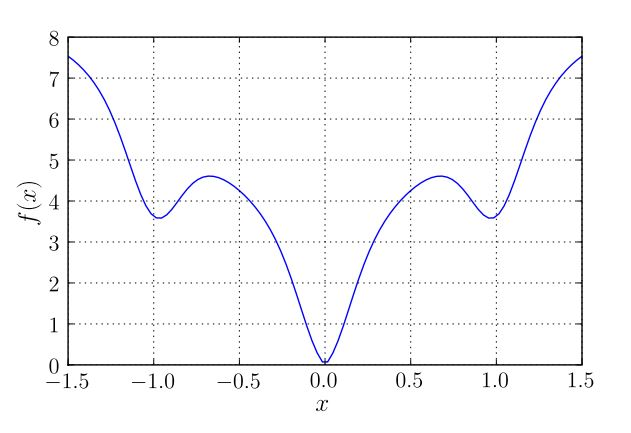
\includegraphics[width=0.9\textwidth]{Figuras/2.TheoryBackground/2-4-2-MultimodalFunction.jpg}}
	\caption{One dimension multi-modal function. Source: \citeonline{Venter}}
	\label{fig:2_4_2_MultimodalFunction}
\end{figure}

A basic form of global optimization is the multi-start approach where multiple local searches are performed. This strategy requires a previous investigation of the design space in order to avoid computational cost by eliminating initial solutions that are to close and will probably converge to the same local minimum. As mentioned, the computational cost of this strategy is very high, in fact, it will be $n$ times the cost of a local algorithm, where $n$ is the number of initial solutions evaluated.

Another form of global optimization are the evolutionary algorithms. These are inspired in observation of organizations found in nature or society. The most popular evolutionary algorithm is the Genetic Algorithm (GA) which was inspired by Darwin's survival of the fittest principle.

Essentially, GA is a population based algorithm where each individual is a design solution. The population evolve iteratively and the solution set of each iteration is called a generation.

The first generation individuals are obtained randomly or through an investigation of the design space and selection of feasible solutions. The following generations are obtained by a process that mimics the reproduction of many living beings. Individuals of a generation are ranked by fitness, given by the objective function, and the best fit are grouped in pairs and called parent designs. The parents are mixed and form children designs in a process called cross-over. Since the population size does not change, each pair makes more than one children. The cross-over is the exchange of genetic material that, in this case, is the mix of characteristics of each solution. 

Additionally to the cross-over, some GA techniques also perform a mutation step which is the random change of characteristics in the individuals of the next generation \cite{Messac}. Mutation increases the possibility of avoiding local minimum because it introduces random changes in population that can place the new individuals in a completely different area of the solution space.

Typical stopping criteria for GA is the number of generations and minimum objective function improvement. The algorithm can yield the best individual of the last generation or its complete set of individuals. The later is useful for multi-objective optimization where a Pareto frontier may be obtained by displaying the best individuals for each objective.

In summary, global optimization techniques are useful for finding global optimum and dealing with discrete design variables. However, it requires the evaluation of a great number of design solutions and this increases its computational cost considerably. It is best suited for problems that do not have a large set of design variables, that are computationally inexpensive, that have discrete variables or problems in which the gradient do not exist.

\subsection{Selected Algorithm} \label{2-4-3-SelectedAlgorithm}

After studying the categories presented in Section \ref{2-3-OptimizationProblems} and understanding the basic characteristics of the most popular optimization algorithms the method employed in this work was selected. 

In this development, the problem is to maximize an actuation system dynamic stiffness through its controller gains while attending several performance requirements. The constraints are the performance requirements and it is a nonlinear problem because the dynamic stiffness and the performance parameters do not have a linear relationship with controller gains. 

Also, these gains are continuous and deterministic variables as well as the internal parameters for the later. Finally, it has a single objective which is to maximize dynamic stiffness but the problem may be stated in a form of multi-objective optimization if there is an objective function for the stiffness at each frequency. Therefore, the problem is constrained, nonlinear, continuous, deterministic and has a single objective.

\citeonline{OptToolbox} presents guidelines for selecting an appropriate algorithm for an optimization problem based on objective and constraint function types. Using these guidelines the interior point method and the \textit{fmincon} solver were selected.

The interior point is a local optimization algorithm for nonlinear constrained problems. Its underlying strategy is to turn the inequality constraints into a barrier function that will penalize the objective function if constraints are not satisfied. Therefore, the minimized function is compound by the objective and the barrier functions. 

Additionally, the algorithm performs two types of step at each iteration. The first, called a Newton step, is a direct step that attempts to satisfy the KKT equations for a linear approximation of the updated objective function. If this step is not possible, a conjugated gradient step is performed. In this case, the approach is to minimize a quadratic approximation of the problem subject to linearized constraints \cite{OptToolbox}. 

The interior point algorithm is executed in MATLAB through the \textit{fmincon} solver. The inputs and outputs parameters of \textit{fmincon} have the following sintax:

\begin{math}
\newline
\centering
[x,fval,exitflag,output] = fmincon(fun,x_0,A,b,A\textsubscript{eq},b\textsubscript{eq},l_b,u_b,nonlcon,options)
\newline
\end{math}

Where:

\begin{description}
	\item \hspace{20pt}$x$: array of design variables of the optimized solution;
	\item \hspace{20pt}$fval$: value of the objective function of the optimized solution;
	\item \hspace{20pt}$exitflag$: parameter that informs trigged stopping criteria;
	\item \hspace{20pt}$output$: structure with information about the optimization process;
	\item \hspace{20pt}$fun$: objective function;
	\item \hspace{20pt}$x_0$: design variables initial values;
	\item \hspace{20pt}$A$: matrix $A$ of $A*x=b$ linear inequality constraint;
	\item \hspace{20pt}$b$: matrix $b$ of $A*x=b$ linear inequality constraint;
	\item \hspace{20pt}$A\textsubscript{eq}$: matrix $A\textsubscript{eq}$ of $A\textsubscript{eq}*x=b\textsubscript{eq}$ linear equality constraint;
	\item \hspace{20pt}$b\textsubscript{eq}$: matrix $b\textsubscript{eq}$ of $A\textsubscript{eq}*x=b\textsubscript{eq}$ linear equality constraint;
	\item \hspace{20pt}$l_b$: lower boundary values for each element of $x$;
	\item \hspace{20pt}$u_p$: upper boundary values for each element of $x$;
	\item \hspace{20pt}$nonlcon$: nonlinear constraint function;
	\item \hspace{20pt}$options$: structure with information to configure \textit{fmincon};
\end{description}

The output parameters inform final design variables, objective function and exit flag. Also, $output$ contains details such as number of iterations and number of function evaluations. 

Input parameters allow definition of $x$ boundaries as well as linear and nonlinear equality and inequality constraints. The nonlinear constraint function must return each evaluated constraint organized in two arrays: one for quality and other for inequality constraints. Other input parameters are the initial values of $x$ and the objective function, that must return a scalar value. Finally, $options$ allow the configuration of stopping criteria tolerances, optimization algorithm, interface and others.


%\section{Frequency Response with Chirp Signal}
%
%The frequency response of a system can be obtained by exciting it with sine waves at each frequency of interest and measuring the output amplitude and phase delay in the steady state using a wave analyzer \cite{Dorf}. 
%
%In a computational environment, this can be achieved by simulating the system with an equal input and processing the output to obtain the amplitude and phase delay at each evaluated frequency. However, in applications with complex models the frequency response test may have a long execution time because of the multiple simulations. 
%
%One alternative to this method is performing the frequency response test with a chirp input instead of a sine wave. A chirp input, shown in Figure \ref{fig:2_4_ChirpSignal} is a sinusoidal wave with time variable frequency, therefore, it can stimulate the system in a range of frequencies in only one simulation. 
%
%
%\begin{figure}[H]
%	\centering
%	\centerline{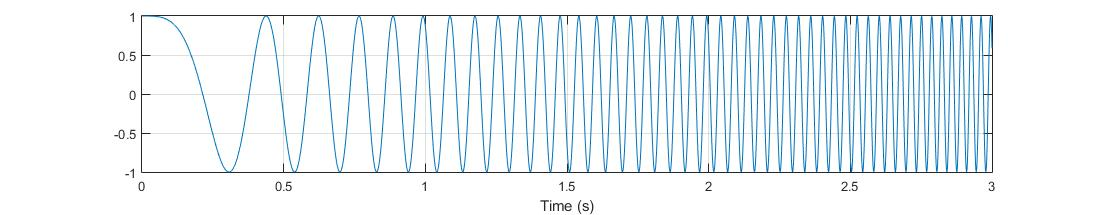
\includegraphics[width=0.9\textwidth]{Figuras/2.TheoryBackground/2-4-Chirp.jpg}}
%	\caption{Chirp Signal}
%	\label{fig:2_4_ChirpSignal}
%\end{figure}
 


